\documentclass{AISB2008}
\usepackage{times}
\usepackage{graphicx}
\usepackage{tabularx,ragged2e}
\usepackage{multirow}
\usepackage{enumerate}
\usepackage{url}
\usepackage[multiple]{footmisc}

% fix table columns
\newcolumntype{Y}{>{\centering\arraybackslash}X}

\begin{document}

\title{Digital Footprints: Envisaging and Analysing\\Online Behaviour}

\author{Giles Oatley \and Tom Crick\institute{Department of Computing, Cardiff Metropolitan
    University, UK; email: \{goatley,tcrick,mmostafa\}@cardiffmet.ac.uk} \and Mohamed
  Mostafa}

\maketitle
\bibliographystyle{AISB2008}

\begin{abstract}
Our long-term research goal is the development of complex (and
adaptive) behavioural modelling and profiling using a multitude of
online datasets; in this paper we look at suitable tools for use in
big social data, specifically here on how to `envisage' this complex
information. We present a novel way of representing personality traits
(using the Five Factor model) with behavioural features (fantasy and
profanity).  We also present some preliminary ideas around developing
a scalable solution to modelling behaviour using swear words.
\end{abstract}


\section{Introduction}

There are large-scale research efforts in developing new and robust
techniques for modelling online behaviour and identity. There exists
numerous domains in which it is essential to obtain knowledge about
user profiles or models of software applications, including
intelligent agents, adaptive systems, intelligent tutoring systems,
recommender systems, e-commerce applications and knowledge management
systems~\cite{schiaffino+amandi:2009}. The rise of Web 2.0 and social
networking has facilitated the publishing of user-generated content on
an exponential scale; its analysis is becoming increasingly important
(and applicable) to the empirical study of society (and thus societal
change).

Big datasets from social networking platforms are now being used for a
multitude of purposes, alongside the obvious advertising, marketing
and revenue generation; increasingly for government monitoring of
citizens\footnote{Twitter Transparency Report 2014:\\
\url{https://transparency.twitter.com/}}\footnote{Facebook Global
Government Requests Report
2014:\\\url{https://govtrequests.facebook.com/}}\footnote{Google
Transparency Report
2014:\\\url{http://www.google.co.uk/transparencyreport/}}, along with
covert security, intelligence community and military user profiling.
However, the publishing of user-generated content on an exponential
scale has significantly changed qualitative and quantitative social
research, with its analysis becoming increasingly important to the
empirical study of society. There are interesting sociological uses of
studying or mining big social data, for instance exploring
cyber-physical crowds using location-tagged social networks or the
study of personality with large-scale benchmark social datasets and
corpora.

However, this ``big social data'' from social media platforms, for
instance social networks, blogs, gaming, shopping and review sites,
differs significantly from more traditional/formal sources.  With the
advent of the social web, there are now orders of magnitude more data
available relating to uncensored natural language, requiring the
development of new techniques that can meaningful analyse it. This
uncensored language is rich in `unnatural' language (as opposed to
`natural' language, used in formal/traditional published media such as
books and newspapers), defined as ``{\emph{informal expressions,
variations, spelling errors...irregular proper nouns, emoticons,
unknown words}}''~\cite{ULPCproc}.  We have been interested in
profiling complex behaviours ~\cite{oatley+crick:2014} and in this
paper we include in our models such bad behaviour that is found in big
social data, for example so-called unnatural language with its poor
language construction but also context dependent acronyms, jargon,
``leetspeak'' and swear words or profanity.  Leet, also known as eleet
or leetspeak, is an alternative alphabet for the English language that
is used primarily on the Internet and in geek/cyber communities. It
uses various combinations of ASCII characters to replace Latin
script. For example, leet spellings of the word ``leet'' include
{\emph{1337}} and {\emph{l33t}}; eleet may be spelled {\emph{31337}}
or {\emph{3l33t}}. See Perea et al.~\cite{perea-et-al:2008} for an
discussion of leet from a cognitive processing perspective.

\section{Modelling Fantasy and Profanity}

\subsection{Rude Words: The Language of Pornography}

A research project investigating opinions on a range of topics related
to pornography usage was carried out; a web-based questionnaire
received over five thousand respondents ({\emph{n}}=5490). Several of
the questions were open-ended, for instance how the person became
involved with the subject of pornography, their particular interests
and so on, eliciting a number of detailed responses (c.2000
words). From the initial findings~\cite{smith-et-al:2013}, the data is
ill-structured, with frequent usage of bad grammar and contains a
large number of jargon (swear) words relating to pornography and
sexuality.

An aim of the original study was the investigation of the usage of
fantasy. This resonated with our general interest in determining
behaviour from data, and so explored the language characteristics of
the answers related specifically to fantasy. We analysed the
respondents text using the psycholinguistic databases LIWC and
MRC. The Dictionary of Affect in Language
(DAL)~\cite{sweeney+whissell:1984} was also planned to be used, due to
its specific uses for imagery-based language. We also used methods
derived from LIWC and MRC to determine personality traits and measures
such as formality and deception. We also wanted to get a general feel
for the level of the text, and to also see if there were any
correlations between literacy and readability.

Initially we focused on the specific questions that might reveal
something about the role of fantasy. For instance, among the many
options for the question ``{\emph{What are your reasons for looking at
pornography?}}'', among the list were the following:

\begin{enumerate}[(A)]
\item ``{\emph{To see things I might do}}'';
\item ``{\emph{To see things I can't do}}'';
\item ``{\emph{To see things I wouldn't do}}'';
\item ``{\emph{To see things I shouldn't do}}''.
\end{enumerate}

The `{\emph{can't}}' and `{\emph{wouldn't}}' choices clearly indicate
respondents utilising pornography more strongly as a form of
fantasy. For this we explored the Five Factors personality traits, in
particular expecting some correlation with the {\emph{Openness to
Experience}} factor (see Figures~\ref{fig:openA}--\ref{fig:openD}.

\begin{table}
\centering
\begin{tabularx}{\columnwidth}{l Y Y Y Y}
%\begin{tabular}{c c c} 
\hline
& A & B & C & D\\ 
\hline
A & 1 &  & & \\
B & -0.72974 & 1 & & \\
C & -0.46635 & -0.06469 & 1 & \\
D & -0.33821 & 0.08321 & 0.091183 & 1\\
\hline
%\end{tabular}
\end{tabularx}
\caption{Correlation between question items (where: A=``{\emph{To
see things I might do}}''; B=``{\emph{To see things I can't do}}''; C=
``{\emph{To see things I wouldn't do}}'' D=``{\emph{To see
things I shouldn't do}}'')}
\label{tbl:abcd}
\end{table}


\begin{figure}[!ht]
\centering
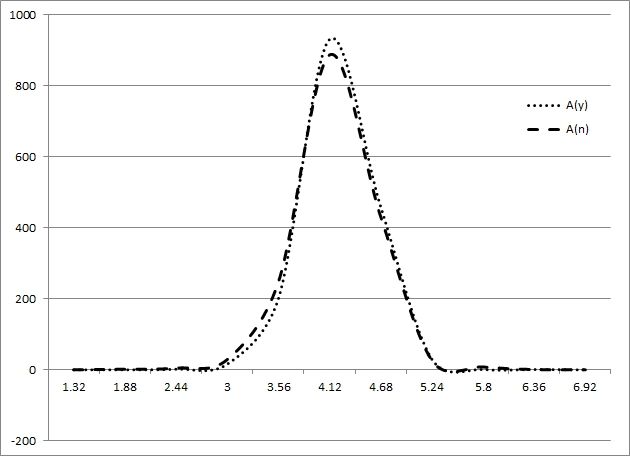
\includegraphics[width=\columnwidth]{images/openA.jpg}
\caption{Openness to experience for A(y) (dotted) versus non-A (dashed)}
\label{fig:openA}
\end{figure}

\begin{figure}[!ht]
\centering
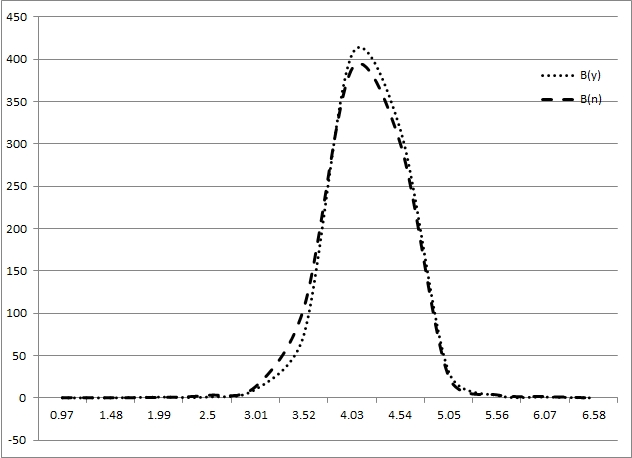
\includegraphics[width=\columnwidth]{images/openB.jpg}
\caption{Openness to experience for B(y) (dotted) versus non-A (dashed)}
\label{fig:openB}
\end{figure}

\begin{figure}[!ht]
\centering
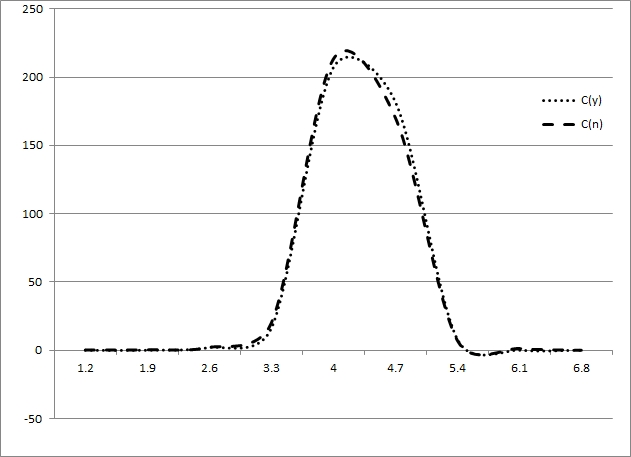
\includegraphics[width=\columnwidth]{images/openC.jpg}
\caption{Openness to experience for C(y) (dotted) versus non-A (dashed)}
\label{fig:openC}
\end{figure}

\begin{figure}[!ht]
\centering
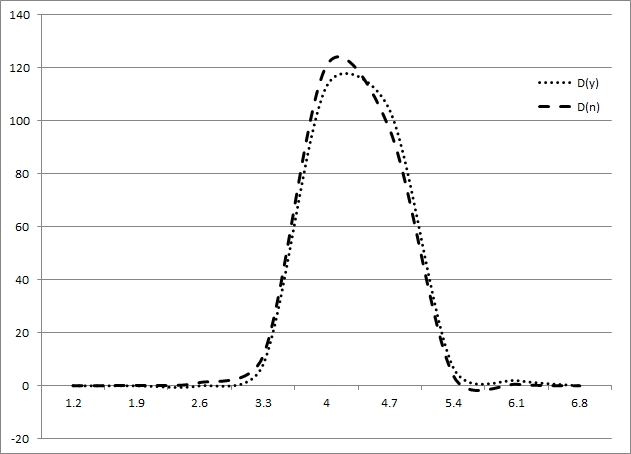
\includegraphics[width=\columnwidth]{images/openD.jpg}
\caption{Openness to experience for D(y) (dotted) versus non-A (dashed)}
\label{fig:openD}
\end{figure}

Analysis is ongoing, with the results to be published in the near
future; however there appears to be a strong negative correlation
between participants who chose ``{\emph{A. To see things I might
do}}'' versus ``{\emph{B. To see things I can't do}}'', as originally
hypothesised. What was less convincing was our analysis of the Five
Factors, and we put this down to the measures we used
from~\cite{mairesse-et-al:2007} being derived from a very different
corpus. We are currently concentrating on the lower level features
from LIWC, MRC and DAL.


\subsection{Disambiguating Profanity}

WordNet\footnote{\url{http://wordnet.princeton.edu/}} is a large
lexical database of English; nouns, verbs, adjectives and adverbs are
grouped into sets of cognitive synonyms (synsets), each expressing a
distinct concept, and each synset is interlinked by means of
conceptual-semantic and lexical relations. Words that are found in
close proximity to one another in the network are semantically
disambiguated. WordNet
Affect\footnote{\url{http://wndomains.fbk.eu/wnaffect.html}}, a
hierarchical set of emotional categories, and
SentiWordNet\footnote{\url{http://sentiwordnet.isti.cnr.it/}}, synsets
are assigned sentiment scores (positivity, negativity, objectivity),
are built on top of WordNet.

Millwood-Hargrave's study~\cite{millwood-hargrave:2000} for Ofcom
(formerly, the Broadcasting Standards Commission), the UK's regulatory
and competition authority for the broadcasting, telecommunications and
postal industries, in 2000 was designed to test people's attitudes to
swearing and offensive language, and to examine the degree to which
context played a role in their reactions. Included in the report was
attitudes towards swearing and offensive language `in life', including
a range of swear words and terms of abuse. Appendix 2's `list of
words' contained positions of the top swear words (categorised as
``{\emph{very severe}}'', ``{\emph{fairly severe}}'', ``{\emph{quite
mild}}'' and ``{\emph{not swearing}}'') and their ranking from 1998 to
2000.

The study of swear words has a longstanding position in linguistics,
with the academic journal {\emph{Maledicta: The International Journal
of Verbal Aggression}} running from 1977 until 2005. Maledicta was
dedicated to the study of the origin, etymology, meaning, use and
influence of vulgar, obscene, aggressive, abusive and blasphemous
language. Unfortunately we do not have resources such as databases in
the literature; furthermore, WordNet does not contain the range of
swear words we encountered in our data and is no use for
disambiguating our text. Wikipedia, however, fared much better; but
even better than these were Roger's Profanisaurus and Urban
Dictionary.

Roger's
Profanisaurus\footnote{\url{http://www.viz.co.uk/profanisaurus.html}}
is a lexicon of profane words and expressions; the 2005 version (the
Profanisaurus Rex), contains over 8,000 words and phrases, with a
further-expanded version released in 2007. Unlike a traditional
dictionary or thesaurus, the content is enlivened by often pungent or
politically incorrect observations and asides intended to provide
further comic effect.

Urban Dictionary\footnote{\url{http://www.urbandictionary.com/}} is a
Web-based dictionary that contains nearly eight million definitions as
of December 2014. Originally, Urban Dictionary was intended as a
peer-reviewed dictionary of slang or cultural words or phrases not
typically found in standard dictionaries, with words or phrases on
Urban Dictionary having multiple definitions, usage examples and tags.

We created different gazetteers related to rude words; one list was
based on Wikipedia entries, and another on lists from Urban
Dictionary. The Wikipedia list was created from link text on the
Wikipedia porn sub-genre
page\footnote{\url{http://en.wikipedia.org/wiki/List_of_pornographic_sub-genres}}
(link ``anchor text'' is a typical approach in semantic relatedness
studies). This was comprised of 250 words. The Urban Dictionary list
was created from the ``sex''
category\footnote{\url{http://www.urbandictionary.com/category/sex}}
(by no means exhaustive -- it is a fraction of the pornography-related
terms in Urban Dictionary). This was comprised of 156 words. We
implemented two metrics for rude words, the key idea of which is to
have a simple mathematical model that enables us to estimate the
life-history value of a token.

There are numerous other lists of pornographic words, which we
compiled from miscellaneous sources; however, we are mainly interested
in sources such as Wikipedia and Urban Dictionary as these are
maintained by a similar community that uses the words in social
networking. In this way we do not have to concern ourselves about this
knowledge engineering process, merely concern ourselves about the
representation and quality of meaning or definitions. We will in
future work make use of the voting scores available on Urban
Dictionary, and look to incorporate new resources such as Roger's
Profanisaurus.


\section{Psycholinguistic Models and Representing Complex Behaviour}

Advances in psychology research have suggested it is possible for
personality to be determined from digital
data~\cite{pennebaker+king:1999,vazire+gosling:2004,iacobelli-et-al:2011}.
Recent studies~\cite{woodworth-et-al:2012} have suggested certain
keywords and phrases can signal underlying tendencies and that this
can form the basis of identifying certain aspects of personality.
Extrapolating this suggests that by investigation of an individual's
online comments it may be possible to identify individual's
personality traits. Initial evidence in support of this hypothesis was
demonstrated in 2012 by analysis of Twitter data for indicators of
psychotic behaviour~\cite{sumner-et-al:2012}. While in the past this
has mainly been the textual information contained in blogs, status
posts and photo comments~\cite{blamey-et-al-2012,blamey-et-al-2013},
there is also a wealth of information in the other ways of interacting
with online artefacts. For instance, it is possible to observe the
ordering/timings of button clicks of a user. Several researchers have
looked at personality prediction (e.g. Five Factor personality traits)
based on information in a user's Facebook
profile~\cite{back-et-al:2010,golbeck-et-al:2001} and
speech~\cite{chung+pennebaker:2007,tausczik+pennebaker:2010}, as well
as also demonstrating significant correlations with fine affect
(emotion) categories such as that of excitement, guilt, yearning, and
admiration~\cite{mohammad+kiritchenko:2013}. There are also several
strands of related work based on the benchmark myPersonality
Project\footnote{\url{http://mypersonality.org/}}
dataset~\cite{celli-et-al:2013}, providing a platform for much-needed
comparative studies.

Mairesse et al.~\cite{mairesse-et-al:2007} highlighted the use of
features from the psycholinguistic databases
LIWC~\cite{pennebaker-et-al:2001} and MRC~\cite{wilson:1988} to create
a range of statistical models for each of the Five Factor personality
traits~\cite{norman:1963,peabody+goldberg:1989}.

In previous work~\cite{oatley+crick:2014} we utilised these methods to
develop a complex behavioural profile that included `two faces' to
model that we can have several different modes of operation (ego
states). We performed our Five Factor analysis, and elaborated two
sets of Five Factor results for each user. We chose Chernoff
faces~\cite{chernoff:1973} for the visual representation. The Five
Factors are displayed as five features on a stylised face, where:

\begin{itemize}
\item Width of hair represents {\emph{Conscientiousness}}; 
\item Width of eyes represents {\emph{Agreeableness}};
\item Width of nose represents {\emph{Openness to experience}}; 
\item Width of mouth represents {\emph{Emotional stability}};
\item Height of face represents {\emph{Extraversion}}.
\end{itemize}

\begin{figure}[!htb]
\centering

\includegraphics[width=\columnwidth]{images/newtwofaces.jpg}
\caption{Two faces of a person. Personality traits from the Five
  Factors model are mapped on a Chernoff face (see later figure for
  specific trait mappings). Two different faces are drawn from two
  different linguistic sources, for the same person.}
\label{fig:twofaces}
\end{figure}

It should be noted that while researchers have continued to work with
the Five Factors model, there are well known
limitations~\cite{eysenck:1992,paunonen+jackson:2000,block:2010} that
are often overlooked by researchers. In particular, it has been
criticised for its limited scope, methodology and the absence of an
underlying theory. However, attempts to replicate the Big Five in other
countries with local dictionaries have succeeded in some countries but
not in others~\cite{szirmak+deraad:1994,defruyt-et-al:2004}. While
\cite{costa+mccrae:1992} claim that their Five Factors model
``represents basic dimensions of personality'', psychologists have
identified important trait models, for instance Cattell's 16
Personality Factors~\cite{cattell:1946} and Eysenck's
biologically-based theory~\cite{eysenck:1947}.


\section{Envisaging Information}

By analysing the myriad approaches of representing complex
information, it is easy to be inspired by Tufte's clarity, precision,
and efficiency~\cite{tufte:2001,tufte:1997,tufte:1990}. We have
integrated the profanity and fantasy behavioural features into our
Chernoff face representing the Five Factor traits -- see
Figure~\ref{fig:blueface} -- represented on a Chernoff face are the
Five Factors plus the additional behaviours for swearing level
(darkness of blue colour on face) and fantasy level (amount of
`thought bubbles').

\begin{figure}[!htb]
\centering
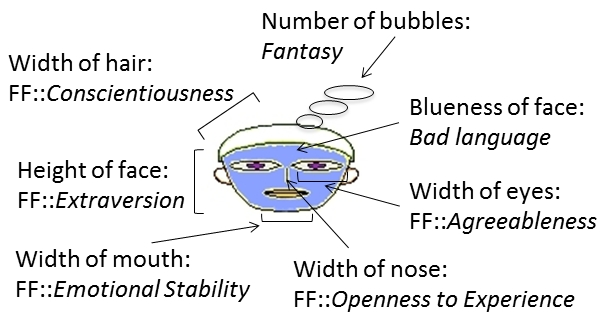
\includegraphics[width=\columnwidth]{images/chernoffnew.jpg}
\caption{Traits and behaviours. Represented on a Chernoff face are the
  Five Factors (prepended by FF::) plus the additional behaviours for
  swearing level (darkness of blue colour on face) and fantasy level
  (amount of `thought bubbles').}
\label{fig:blueface}
\end{figure}


\subsection{Modelling Timelines}

Elsewhere we have presented ways to fuse social network (graph)
information with geographical
information~\cite{oatley-et-al:2006,oatley+crick-gisruk2015}, and from
spatial statistics there exists methods for space and time such as the
Knox and Mantel indices. In this section we look at a method to
represent temporal events, something very necessary when developing a
behavioural profile.

Our data comes from an online portal for a European Union (EU)
international scholarship mobility hosted at a UK university. The case
study looked at how people interact with complex online information
systems, the online portal for submitting applications. We analysed
the document uploading behaviour (also motivation letters, and social
media interactions) of the applicants. By examining the upload
footprint for the users we determined several classes of behaviour.

There were several thousand applications submitted by over a thousand
candidates, applying to 10 EU universities and 10 non-EU
universities. Each mobility call has an opening date/time and closing
date/time, with occasional extensions given for specific reasons (for
instance due to administrative reasons or technical issues with the
portal). Applicants are required to submit for their application
certain mandatory files, such as motivation letter,
passport/identification, curriculum vitae), as well as optional files
(supporting documents).

We simplified an applicant's interaction, or timeline, with the portal
to include the following milestones: {\emph{T0}} Registration Time;
{\emph{T1}} First Action; {\emph{T2}} Last Action; and, {\emph{T3}}
Submission. Additionally we represented an extension to the submission
deadline as {\emph{T4}} Extension. In this way we can represent an
applicants’ interaction as shown in Figure~\ref{fig:timelines}, which
shows seven example timelines.

\begin{figure}[!ht]
\centering
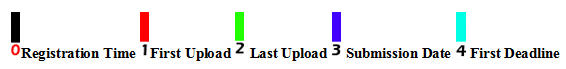
\includegraphics[width=\columnwidth]{images/legend.jpg}
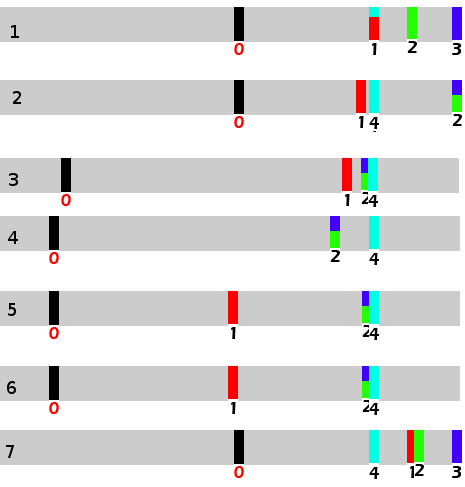
\includegraphics[width=\columnwidth]{images/timelines.jpg}
\caption{Seven user timelines. {\emph{T0}} (black bar) is when the applicant first
registered with the call. {\emph{T1}} (red bar) represents when the applicant
uploaded their first document, or First Action. {\emph{T2}} (green bar)
represents an applicants' Last Action. {\emph{T3}} (blue bar) represents the
applicants' Submission. {\emph{T4}} (aquamarine bar) represents the first
deadline (certain calls had initial deadlines extended).}
\label{fig:timelines}
\end{figure}

Using these milestones we are able to identify interesting behaviours
that compare and contract with personality traits and other sources of
information. Behaviours such as: how long it was before an applicant
became aware of the call, and when they registered; how long after
registration did the applicant carry out their first action with the
system; how long did they take to complete their application; and, how
close to the deadline did they submit their application.

The complete timeline from opening to final close was 125 days. There
was an extension from day 112 until day 125. We divided the timeline
of the call into five equally spaced segments (S0-S4).

Using these segments we were able to assign the various applicant
actions ({\emph{T0}} Registration, {\emph{T1}} First Upload,
{\emph{T2}} Last Upload, {\emph{T3}} Submission) to various time
periods. This allowed us to assign applicants to statistically
significant categories, and also to add in a few categories from
observations. These are shown in the following
Table~\ref{tbl:apptlseg}; as you can see, a small number of applicants
({\emph{n}}=4) registered within the segment S1 (20-40\% of timeline),
and then uploaded all of their documents and submitted within the
segment S3 (60-90\% of timeline). This is represented by Class A, the
first row. Successive rows can be interpreted in the same manner.

\begin{table}[!ht]
\centering
\begin{tabularx}{\columnwidth}{Y Y Y Y Y Y}
%\begin{tabular}{c c c} 
\hline
Class & {\emph{n}} & {\emph{T0}} & {\emph{T1}} & {\emph{T2}} & {\emph{T3}} \\ 
\hline
{\emph{A}} & 4 & S1 & S3 & S3 & S3\\
{\emph{B}} & 14 & S2 & S2 & S2 & S2\\
{\emph{C}} & 128 & S2 & S3 & S3 & S3\\
{\emph{D}} & 29 & S2 & S3 & S4 & S4\\
{\emph{E}} & 678 & S3 & S3 & S3 & S3\\
{\emph{F}} & 202 & S3 & S3 & S4 & S4\\
{\emph{G}} & 9 & S3 & S4 & S4 & S4\\
{\emph{H}} & 54 & S4 & S4 & S4 & S4\\
\hline
%\end{tabular}
\end{tabularx}
\caption{Applicants' timeline actions assigned to segments}
\label{tbl:apptlseg}
\end{table}

\begin{table*}[!htb]
\centering
\begin{tabularx}{\textwidth}{c X l}
%\begin{tabular}{c c c} 
\hline
Class & Description & Potential Alias  \\ 
\hline
{\emph{A}} & Register early, and take some time to upload documents, but submit with plenty of time before deadline & EverythingEarly\\
{\emph{B}} & Register reasonably early, but then upload documents and submit straight after with plenty of time before deadline, making no amendments & QuiteEarlyAndQuick\\
{\emph{C}} & Similar to Class B, but submitting more slowly & Cautious\\
{\emph{D}} & Registers reasonably early, and then takes time to upload, and only submits at the last days & VeryCautious\\
{\emph{E}} & Latecomer to registration, but then uploads and submits
quickly thereafter & Cautious\\
{\emph{F}} & Latecomer to registration, but then uploads and submits
slowly & Cautious\\
{\emph{G}} & Latecomer to registration, but delays uploading and
submission to last days & Cautious\\
{\emph{H}} & Does everything at the last days, from registration to submission & EverythingLastMinute\\
\hline
%\end{tabular}
\end{tabularx}
\caption{Description of each class}
\label{tbl:classdesc}
\end{table*}

We did not want to ascribe a premature alias to the behaviours, as we
recognise that there are several possible interpretations;
nevertheless, we have used the `Potential Alias' column in
Table~\ref{tbl:classdesc} to indicate some initial thoughts.

Combining this information with the earlier trait and behaviour model,
it could be possible to present several faces along the timeline, or
to represent the temporal aspect as a 'clock-type' metaphor, the
straight line curved around, surrounding the face.  The latter would
perhaps be preferable, as we would expect that traits persist through
time, but behaviours change. Likewise we would expect the blueness
(rudeness) of the Chernoff face to change, and the amount of bubbles
(fantasy) to change, but the facial features to remain constant
(personality traits).

\section{Conclusions and Future Work}

The linguistic methods for determining personality traits are still in
their infancy, and we have already noted some of the opposition to the
lexical hypothesis~\cite{block:2010}. We would expect that in time
additional information sources, like how people project identities
through personal websites~\cite{vazire+gosling:2004}, judging people
by their music preferences~\cite{rentfrow+gosling:2006},
personalisation of workspaces~\cite{wells+thelen:2002}, etc, will all
help with classification.

Further problems related to using social media for classification are
that existing NLP tools are known to struggle with unnatural language:
``{\emph{demonstrated that existing tools for POS tagging, chunking
and Named Entity Recognition perform quite poorly when applied to
tweets}}''~\cite{ritter-et-al:2011} and ``{\emph{showed that
[lengthening words] is a common phenomenon in
Twitter}}''~\cite{brody+diakopoulos:2011}, presenting a problem for
lexicon-based approaches. These investigations both employed some form
of inexact word matching to overcome the difficulties of unnatural
language. We have made no attempt to use inexact string matching or to
make use of a leetspeak parser. This will form part of future work.

To assist with the ongoing knowledge modelling problem in this domain
we recognise the need to utilise specific lexicons that keep pace with
the language used, for instance the use of Urban Dictionary to resolve
swear words. We need to study how in what precise manner this resource
keeps pace with popular culture.

\bibliography{aisb2015}

\end{document}





